\documentclass{scrartcl}
\usepackage[T1]{fontenc}
\usepackage[utf8]{inputenc}
\usepackage[ngerman]{babel}
\usepackage{amsmath,amssymb}
\usepackage{graphicx}
\usepackage{enumerate}

\begin{document}
\section*{Aufgaben zum Thema Datenstrukturen}
\begin{enumerate}[(1)]

\item
\begin{enumerate}[(a)]
\item Geben sie f\"ur $n\in \{0,1,2,3,4\}$ alle M\"oglichkeiten an, die Zahlen $1,\dots,n$ in einen Min-Heap einzuordnen. Der Heap soll minimale H\"ohe haben und ein rechter Unterbaum darf nicht h\"oher sein als ein linker Unterbaum desselben Knotens.
\item Welche Heaps aus (a) haben in der Arraydarstellung keine L\"ucken?
\item Stellen Sie den folgenden Heap als Array dar. Verwenden Sie $\bot$, um L\"ucken zu kennzeichnen:\newline
{\center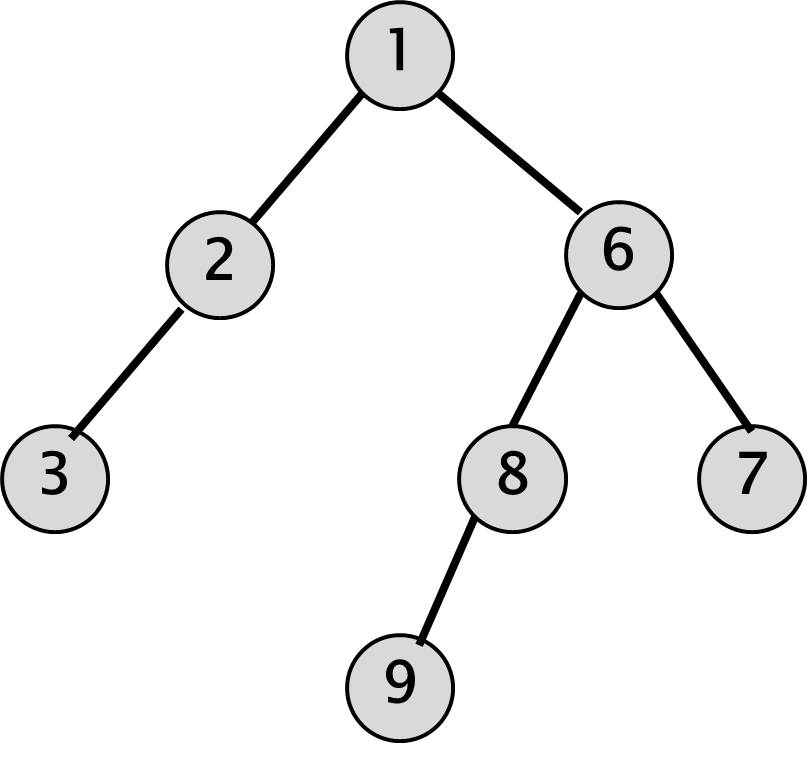
\includegraphics[scale=0.3]{Heap.jpg}}
\end{enumerate}

\item
Gesucht ist eine Datenstruktur, in der Einf\"ugen in konstanter Zeit ebenso m\"oglich ist wie die R\"uckgabe des minimalen Werts.
\begin{enumerate}[(a)]
\item Beschreiben Sie kurz eine m\"ogliche Datenstruktur.
\item Schreiben Sie Pseudocode f\"ur das Einf\"ugen. Es gen\"ugt, den f\"ur die sp\"atere R\"uckgabe des Minimums relevanten Teil zu betrachten.
\item Schreiben Sie Pseudocode, der das Minimum zur\"uckgibt.
\item Beschreiben Sie kurz, was beim Entfernen eines Elements passieren muss. Hat dies Auswirkung auf die Laufzeit des L\"oschens?
\end{enumerate}

\item Für die folgenden Anwendungsfälle soll jeweils eine geeignete Datenstruktur ausgewählt werden. Geben Sie jeweils eine passende Datenstruktur an und begründen Sie Ihre Wahl:
\begin{enumerate}[(a)]
\item In einer Musiksammlung sollen häufig neue Musikstücke hinzugefügt, gelöscht und gesucht werden. Über die zukünftige Größe der Sammlung kann beim Anlegen noch keine Aussage gemacht werden.
\item An einen Datenbankserver werden zu manchen Zeitpunkten so viele Anfragen geschickt, dass er sie nicht sofort bearbeiten kann. Daher soll er die Möglichkeit bekommen, die Anfragen zwischenspeichern zu können, bis er wieder genügend freie Ressourcen besitzt.
\item Ein Prozess-Scheduler in einem Betriebssystem arbeitet mit unterschiedlich hohen Prioritäten. Bei jedem Aufruf soll jeweils der Prozess mit der höchsten Priorität ausgeführt werden, wobei die Auswahlgeschwindigkeit für die Leistungsfähigkeit des Betriebssystems eine entscheidende Rolle spielt.
\end{enumerate}

\item Zeigen Sie, wie eine Warteschlange mit einer \textbf{einfach verketteten} Liste sowie zwei Zeigern \textit{K} (ältestes Element) und \textit{E} (neuestes Element) implementiert werden kann. Hierbei sollen sowohl ENQUEUE(X) als auch DEQUEUE() die Laufzeit O(1) besitzen.\\
Gehen Sie dafür folgendermaßen vor:\\
\begin{itemize}
	\item Stellen Sie mit einer Skizze dar, wie die beiden Zeiger in der Liste positioniert werden müssen.
	\item Geben Sie den Pseudocode für beide Warteschlangenoperationen an. Stellen  Sie dabei sicher, dass Ihre Implementierung auch korrekt mit einer leeren Warteschlange umgehen kann.
\end{itemize}

\end{enumerate}
\end{document}